\section{Do bar-based proxies measure what they claim?}\label{sec:validation}

This section scores the OHLCV-only measures against the quantities they are meant to capture.
Observed signed flow is the taker imbalance $(2B_t-V_t)/V_t$; the benchmark for volatility is
realised variance from one-minute returns. Because quoted spreads are not in the public archive, we
evaluate the spread estimators indirectly, against the tick size and against volatility.
Table~\ref{tab:validation} collects the main statistics for BTC/USDT; ETH/USDT results are in
Appendix Table~\ref{tab:validation_eth}.

\begin{table}[t]
\centering\caption{Bar-based proxies against observed quantities, BTC/USDT}\label{tab:validation}
\resizebox{\textwidth}{!}{\begin{tabular}{lrrrr}
\toprule
 & Pearson & Spearman & Same sign & $N$\\
\midrule
\multicolumn{5}{l}{\emph{Panel A. Signed order flow: proxy vs.\ observed taker imbalance}}\\
BVC, 1h bars, per hour & 0.489 & 0.541 & 0.716 & 42,316\\
BVC, 1h bars, 4h sums & 0.475 & 0.524 & 0.701 & 42,310\\
BVC, 1h bars, 24h sums & 0.507 & 0.538 & 0.693 & 42,270\\
BVC, 1m bars summed to 1h & 0.603 & 0.637 & 0.747 & 42,359\\
Tick rule, 1h bars, per hour & 0.430 & 0.389 & 0.716 & 42,357\\
\midrule
\multicolumn{5}{l}{\emph{Panel B. Price impact and volatility}}\\
Kyle $\lambda$ (48h): BVC vs.\ observed flow & 0.260 & 0.213 & -- & 41,978\\
log GK vol (1h bars) vs.\ log RV (1m), 24h & 0.987 & 0.983 & -- & 41,978\\
\midrule
\multicolumn{5}{l}{\emph{Panel C. Information ceiling of return-based classifiers (out-of-sample $R^2$)}}\\
 & BVC raw & BVC rescaled & Any $f(z)$ & $N$\\
1h bars & \ensuremath{-}6.783 & 0.209 & 0.213 & 21,158\\
1m bars & 0.116 & 0.308 & 0.328 & 1,270,544\\
\midrule
\multicolumn{5}{l}{\emph{Panel D. Spread estimators (one tick $=$ 0.002 bps)}}\\
 & Median (bps) & Mean (bps) & Share $=0$ & Corr.\ log RV\\
Corwin-Schultz (24h mean) & 15.8 & 17.5 & 0.0\% & 0.87\\
Abdi-Ranaldo (24h) & 0.0 & 9.6 & 50.2\% & 0.64\\
Roll (48h) & 15.1 & 19.7 & 38.4\% & 0.52\\
\bottomrule
\end{tabular}
}
\tabnote{Panel A: correlation and sign agreement between proxy and observed taker imbalance
$(2B_t-V_t)/V_t$, per hour and over rolling 4- and 24-hour sums. Panel B: Kyle's lambda from 48-hour
rolling regressions on BVC-signed and on observed signed dollar volume; Garman-Klass volatility from
hourly bars against realised volatility from one-minute returns. Panel C: out-of-sample $R^2$ for
observed imbalance of raw BVC, of BVC after a linear rescaling, and of the best function of the
standardised bar return (50 quantile bins), all fitted on the first half and evaluated on the second.
Panel D: spread estimators in basis points, share of hours truncated at zero, and correlation of the
log estimate with log realised volatility.}
\end{table}

\paragraph{Signed order flow.} Hourly BVC imbalance has a correlation of \BTCbvcCorr{} with observed
taker imbalance and the same sign in \BTCbvcSign{} of hours. Aggregating to 24 hours barely changes
the correlation (\BTCbvcCorrDay), so the error is not high-frequency noise that averages out. Applying
BVC to one-minute bars and summing within the hour raises the correlation to \BTCbvcOneMinCorr{}, the
largest gain available from the data we use. The choice of the volatility window (24 hours to
30 days) or of a heavy-tailed Student-$t$ CDF moves the correlation by at most two hundredths
(Appendix Table~\ref{tab:variants}). The tick rule, which signs the whole bar by its return, is
worse on hourly bars but nearly as good as BVC on one-minute bars, consistent with
\citet{chakrabarty2015} and \citet{panayides2019}.

\paragraph{An information ceiling for return-based classification.} BVC, the tick rule and their
variants are all functions of the standardised bar return $z_t=r_t/\hat\sigma_t$. Their accuracy is
therefore bounded by how much of the observed imbalance is explained by $\mathbb E[\text{imb}_t\mid
z_t]$, whatever the functional form. We estimate this conditional mean nonparametrically with 50
quantile bins of $z_t$. As an upper bound we compute its in-sample $R^2$; with 50 bins and
thousands of hours per period the overfitting bias is negligible. Over the full sample the bound is
\BTCceilIS{} on hourly bars and \BTCceilISm{} on one-minute bars, and in no calendar year does the
hourly bound exceed \BTCceilISmax{} (Appendix Table~\ref{tab:ceiling}). The squared correlation of
BVC with observed imbalance is \BTCcorrsqBVC, almost exactly at the bound: the shape of the BVC map
is close to optimal, and no other function of the bar return would do materially better. Fitted on
the first half of the sample and evaluated on the second, the out-of-sample ceiling is \BTCceilH, and
rescaled BVC attains \BTCbvcResH. Fitted on the second half and evaluated on the first, however, it falls to
\BTCceilRev{} for BTC (\ETHceilRev{} for ETH), because the scale of the relation drifts: the slope
of observed imbalance on BVC rises from \BTCslopeFirst{} in 2022 to \BTCslopeLast{} in 2026. A
classifier calibrated in one period is therefore miscalibrated in another, so out-of-sample
accuracy is lower than the bound.

Figure~\ref{fig:calibration} shows the mechanism. The BVC map $2\Phi(z)-1$ has the right shape, but
observed imbalance moves far less than the map implies (the slope fitted on the first half of the
sample is \BTCslopeH{} on hourly bars), and its dispersion at any given return is wide. Two conclusions follow. First, the shape of
the classifier is not the problem; recalibration, which \citet{panayides2019} recommend, fixes the
scale but must be repeated as the scale drifts. Second, about three-quarters of the hourly variation
in aggressor imbalance leaves no trace in the bar's own price change. This flow is absorbed by
passive liquidity, offset within the hour, or reflected in prices only later, and no classifier
based on the hourly bar can recover it. Part of it is visible in the one-minute price path, which is
why BVC on one-minute bars does better.

\begin{figure}[t]
\centering
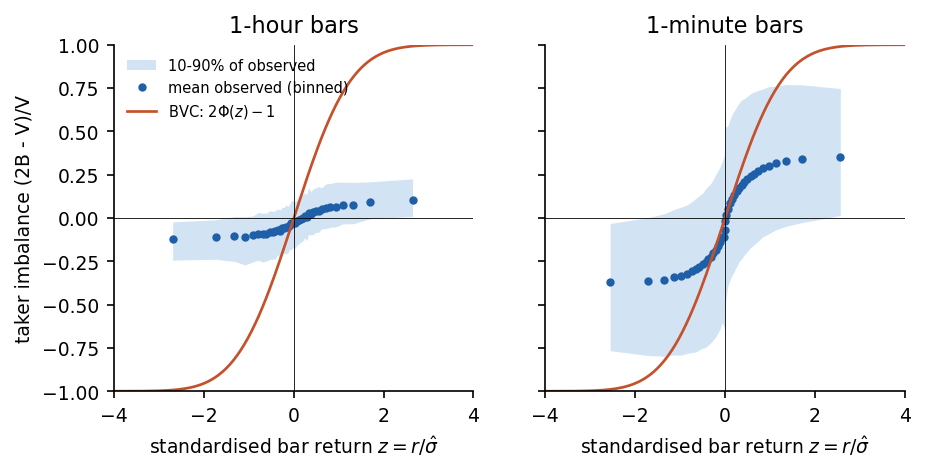
\includegraphics[width=0.85\textwidth]{fig_bvc_calibration.png}
\caption{Observed taker imbalance against the standardised bar return. Dots are bin means of
observed imbalance in 40 quantile bins of $z$; the band covers the 10th to 90th percentile within
each bin; the line is the BVC mapping $2\Phi(z)-1$. BTC/USDT, January 2022 to October 2026.}
\label{fig:calibration}
\end{figure}

\paragraph{Price impact.} Kyle's lambda estimated from BVC-signed dollar volume has a correlation of
only \BTClambdaCorr{} with the same estimator applied to observed signed volume. Errors in the
regressor are amplified in a ratio of a covariance to a variance, so a proxy that captures about
a quarter of the flow variance yields an impact estimate that is largely noise.

\paragraph{Volatility.} The range-based Garman-Klass estimator from hourly bars has a correlation
of \BTCgkCorr{} with realised variance from one-minute returns (both in logs, 24-hour windows).
Bar-based volatility measures are close substitutes for realised measures at this horizon.

\paragraph{Spreads.} The minimum quoted spread on BTC/USDT is one tick of 0.01~USDT, about
\BTCtick{} basis points at the sample's median price. The 24-hour Corwin-Schultz estimate has a median
of \BTCcsMedian{} basis points, so taken at face value it would imply an average book about four
orders of magnitude wider than one tick, an implausible value for the most liquid crypto pair. Its
logarithm has a correlation of \BTCcsVolCorr{} with log realised volatility. The Abdi-Ranaldo
estimate is truncated at zero in \BTCarZero{} of hours and the Roll estimate in \BTCrollZero. In this
market the spread estimators measure volatility, the extreme case of the bias documented by
\citet{jahanparvar2023}. Liquidity conclusions drawn from them at hourly frequency should be read as
volatility conclusions.

\paragraph{Stability.} The BVC correlation varies between \BTCbvcYearMin{} and \BTCbvcYearMax{}
across calendar years and is essentially the same in low-, medium- and high-volatility regimes at
the hourly level (Appendix Table~\ref{tab:regimes}). It is higher during Binance's zero-fee
promotion on BTC/USDT (8 July 2022 to 22 March 2023), when hourly trade counts rose sharply
(\BTCbvcZeroFee{} against \BTCbvcStdFee{} under standard fees). The reason is visible in the
flow itself. During the promotion the standard deviation of hourly taker imbalance on BTC/USDT fell
to \BTCsdImbZero, from \BTCsdImbStd{} under standard fees: volume rose fivefold but became almost
perfectly two-sided, which is what costless round-trip trading produces. On ETH/USDT, which kept its
fees, the dispersion barely changed (\ETHsdImbZero{} against \ETHsdImbStd). With little genuine
directional flow left, the price change of a bar explains a larger share of what remains. The
relation between prices and aggressor flow therefore depends on the exchange's fee schedule and on
the composition of trading it attracts \citep{cong2023}, and data from fee-free periods should be
treated with care.
